\documentclass[9pt,twoside]{pnas-new}

\templatetype{pnasmathematics} 

\usepackage{pdfpages}
\usepackage{subfigure}

\title{Machine Learning based Recommender System in Social Networks}

% Authors should be listed in alphabetical order by last name. Use letters to indicate affiliations.
\author[a]{Albert Jian} 
\author[a]{Bill Wen}
\author[a]{Shan Zhong}

\affil[a]{University of California, Los Angeles}

% Please give the surname of the lead author for the running footer
\leadauthor{Zhong} 

% Please add a significance statement to explain the relevance of your work
\significancestatement{Given a social network, how can you predict and recommend a likely future friendship between two users? Here, we design a recommender system based on machine learning with features to represent similarity with different properties each.}

% Please include author contributions here.
\authorcontributions{Please provide details of author contributions here.}

% Please provide three to five keywords, separated by the pipe symbol. Keywords will signal the application, methods, etc. to the reader.
\keywords{Machine Learning $|$ Recommender System $|$ Social Networks } 

\begin{abstract}
Recommender systems attempts to predict a user's rating on an item based on available data. In the context of social networks, recommender systems recommends a likely acquitance to a user. In this paper, we use similarity measures from network theory to develop features for machine learning to produce a recommender system. Using training and testing sets, we are able to demonstrate a system with accuracy.
\end{abstract}

\dates{This manuscript was compiled on \today}
\doi{Math 168 Spring 2020 Final Project}

\newcommand\boldred[1]{\textcolor{red}{\textbf{#1}}}

\begin{document}

\maketitle
\thispagestyle{firststyle}
\ifthenelse{\boolean{shortarticle}}{\ifthenelse{\boolean{singlecolumn}}{\abscontentformatted}{\abscontent}}{}

% If your first paragraph (i.e. with the \dropcap) contains a list environment (quote, quotation, theorem, definition, enumerate, itemize...), the line after the list may have some extra indentation. If this is the case, add \parshape=0 to the end of the list environment.
\dropcap{R}ecommender systems is prevalently used in companies to give the best and personalized recommendations to users. In social networks, it can be 

\section*{Dataset}
The dataset GitHub Social Network is taken from SNAP. \cite{rozemberczki2019multiscale}. This dataset contains a large social network of GitHub developers, with each node representing a developer with at least 10 starred repositories and each edge indicating a mutual follower relationship.
\subsection*{Data Analysis}
\boldred{Some insight on how our network looks and behave}

\begin{figure}%[tbhp]
    \centering
    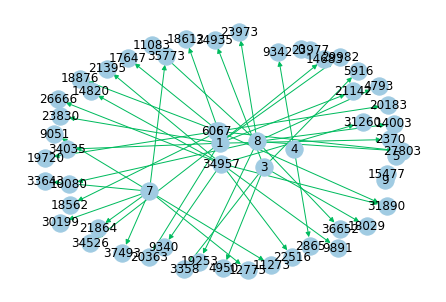
\includegraphics[width=.8\linewidth]{Figures/subgraph.png}
    \caption{Followers subgraph}
    \label{fig:followers_subgraph}
\end{figure}

\begin{figure}%[tbhp]
    \centering
    \subfigure[Mutual follows for all users]{
        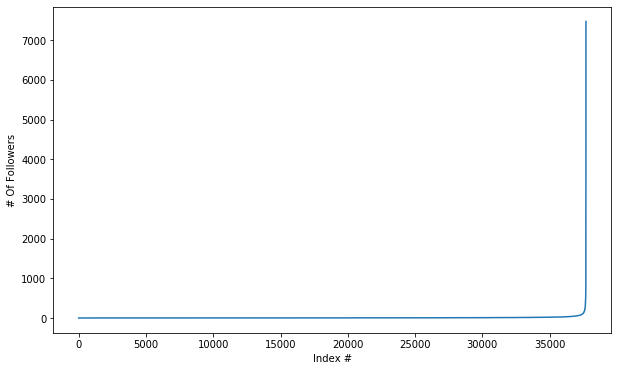
\includegraphics[width=0.3\textwidth]{Figures/followers_overall.png}
    }
    \subfigure[Mutual follows for the least 30000 users]{
        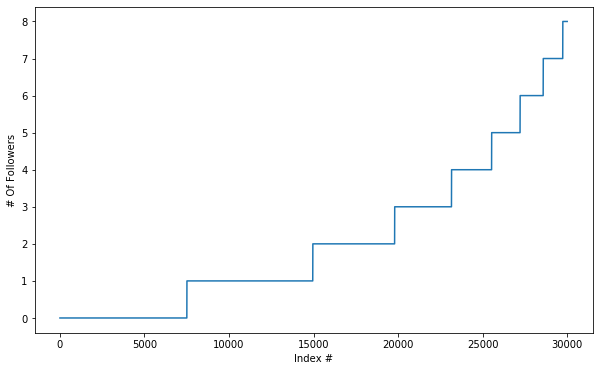
\includegraphics[width=0.3\textwidth]{Figures/followers_30000.png}
    }
    \subfigure[Mutual follows box plot]{
        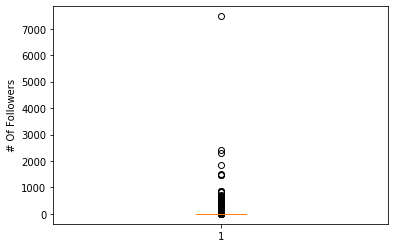
\includegraphics[width=0.3\textwidth]{Figures/followers_boxplot.png}
    }
    \caption{Mutual follows per user}
    \label{fig:followers}
\end{figure}

\begin{figure}%[tbhp]
    \centering
    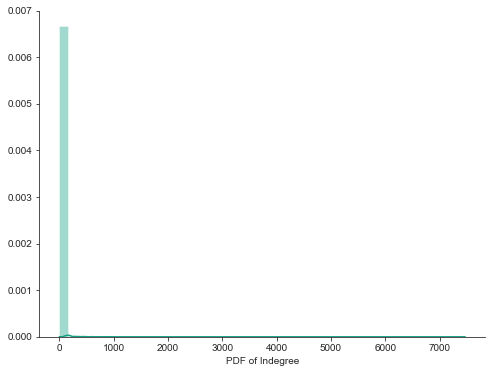
\includegraphics[width=.8\linewidth]{Figures/followers_pdf.png}
    \caption{Followers pdf}
    \label{fig:followers_pdf}
\end{figure}

\section*{Methods}
We use machine learning with features from similarity measures and other weighted measures\cite{6033365}.

\subsection*{Features}

\subsubsection*{Jaccard's Coefficient}
\subsubsection*{Preferential Attachment}
\cite{sadraei}
\section*{Results}
The results are quite convincing, as indicated in the confusion matrices \ref{fig:pa_train_confusion_matrix},\ref{fig:pa_test_confusion_matrix},\ref{fig:pa_roc_curve}



\begin{figure}%[tbhp]
    \centering
    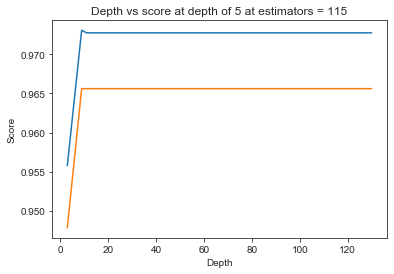
\includegraphics[width=.8\linewidth]{Figures/mt_depth_score.png}
    \caption{Placeholder image of a frog with a long example legend to show justification setting.}
    \label{fig:mt_depth_score}
\end{figure}

\begin{figure}%[tbhp]
    \centering
    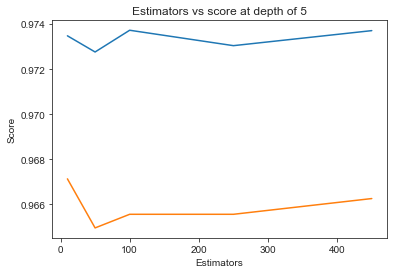
\includegraphics[width=.8\linewidth]{Figures/mt_estimator_score.png}
    \caption{Placeholder image of a frog with a long example legend to show justification setting.}
    \label{fig:mt_estimator_score}
\end{figure}

\begin{figure}%[tbhp]
    \centering
    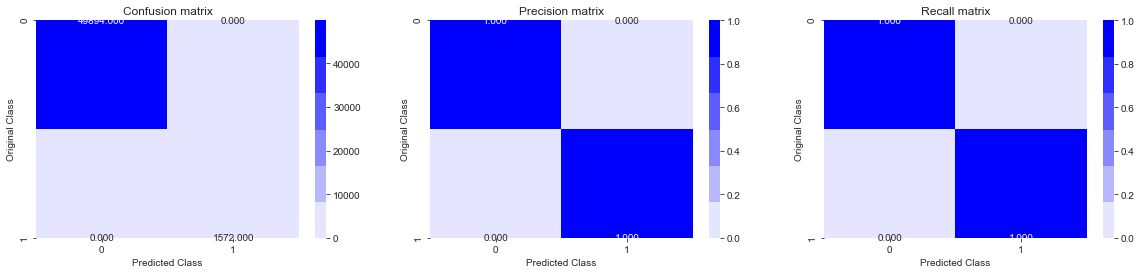
\includegraphics[width=.8\linewidth]{Figures/pa_train_confusion_matrix.png}
    \caption{Placeholder image of a frog with a long example legend to show justification setting.}
    \label{fig:pa_train_confusion_matrix}
\end{figure}

\begin{figure}%[tbhp]
    \centering
    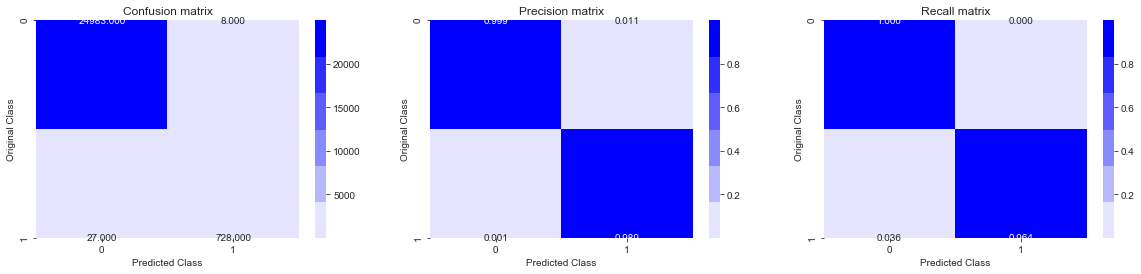
\includegraphics[width=.8\linewidth]{Figures/pa_test_confusion_matrix.png}
    \caption{Placeholder image of a frog with a long example legend to show justification setting.}
    \label{fig:pa_test_confusion_matrix}
\end{figure}

\begin{figure}%[tbhp]
    \centering
    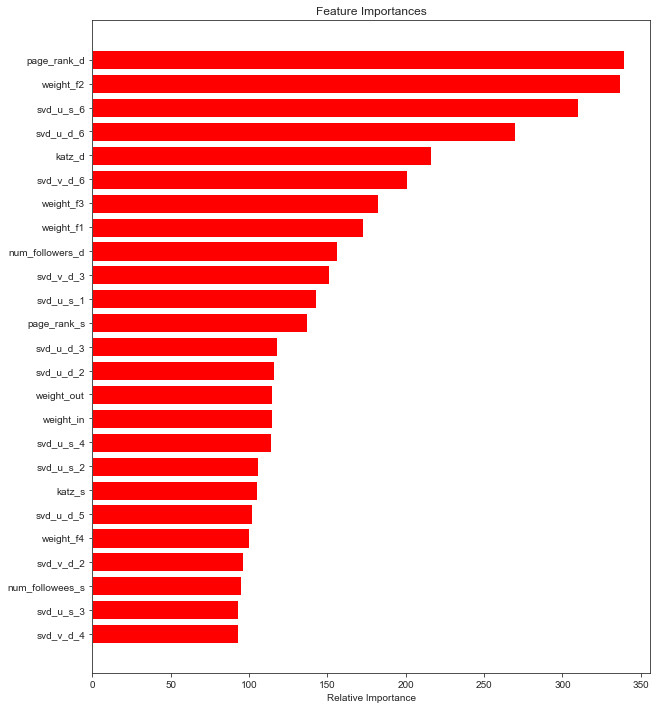
\includegraphics[width=.8\linewidth]{Figures/pa_feature_importance.png}
    \caption{Placeholder image of a frog with a long example legend to show justification setting.}
    \label{fig:pa_feature_importance}
\end{figure}

\begin{figure}%[tbhp]
    \centering
    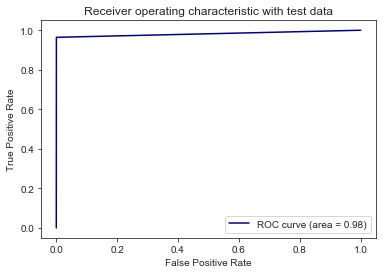
\includegraphics[width=.8\linewidth]{Figures/pa_roc_curve.png}
    \caption{Placeholder image of a frog with a long example legend to show justification setting.}
    \label{fig:pa_roc_curve}
\end{figure}

\section*{Supporting Information}

\acknow{If you wish, you can include any acknowledgments here, set in a single paragraph.}

\showacknow % Display the acknowledgements section

% Bibliography
\bibliography{References}

\clearpage
\includepdf[
    %% Include all pages of the PDF
    pages=-,
    %% make this page have the usual page style
    %% (you can change it to plain etc). By default pdfpages
    %% sets the pagecommand to \pagestyle{empty}
    pagecommand={\pagestyle{headings}},  
    %% Add a "section" entry to the ToC with the heading
    %% "Quilling Shapes" and the label "sec:shapes"
    addtotoc={1,section,1,Quilling Shapes,sec:shapes}]
%% The pdf file itself
{Math168_Final_Project.pdf}

\end{document}
